%%%%%% CMB-S4 Simulations and Data Analysis Chapter, Data Simulation Section  %%%%%%%%%%%%%%%%
 
\section{Data Simulation}

The data simulation subset of the CMB simulation pipeline (Figure \ref{fig_ds}) takes the sky model and applies the mission model to it to generate a simulated data set for that mission. The mission model consists of two parts; the instrument model defines the data acquisition system (telescope, detectors, read-out), while the observation model defines its deployment (scanning strategy, environment). Depending on the degree of detail of the sky, instrument and observation model that we include, the resulting data set can be in any of the data domains - time-ordered (raw or clean), map, or spectral. Inevitably there is a trade-off between the realism of the simulation and the complexity and cost both of generating the model inputs and of performing the simulation, with the choice reflecting both the requirements of the subsequent analyses of the data set and the availability of computational resources.

\begin{figure}[htbp]
\centering
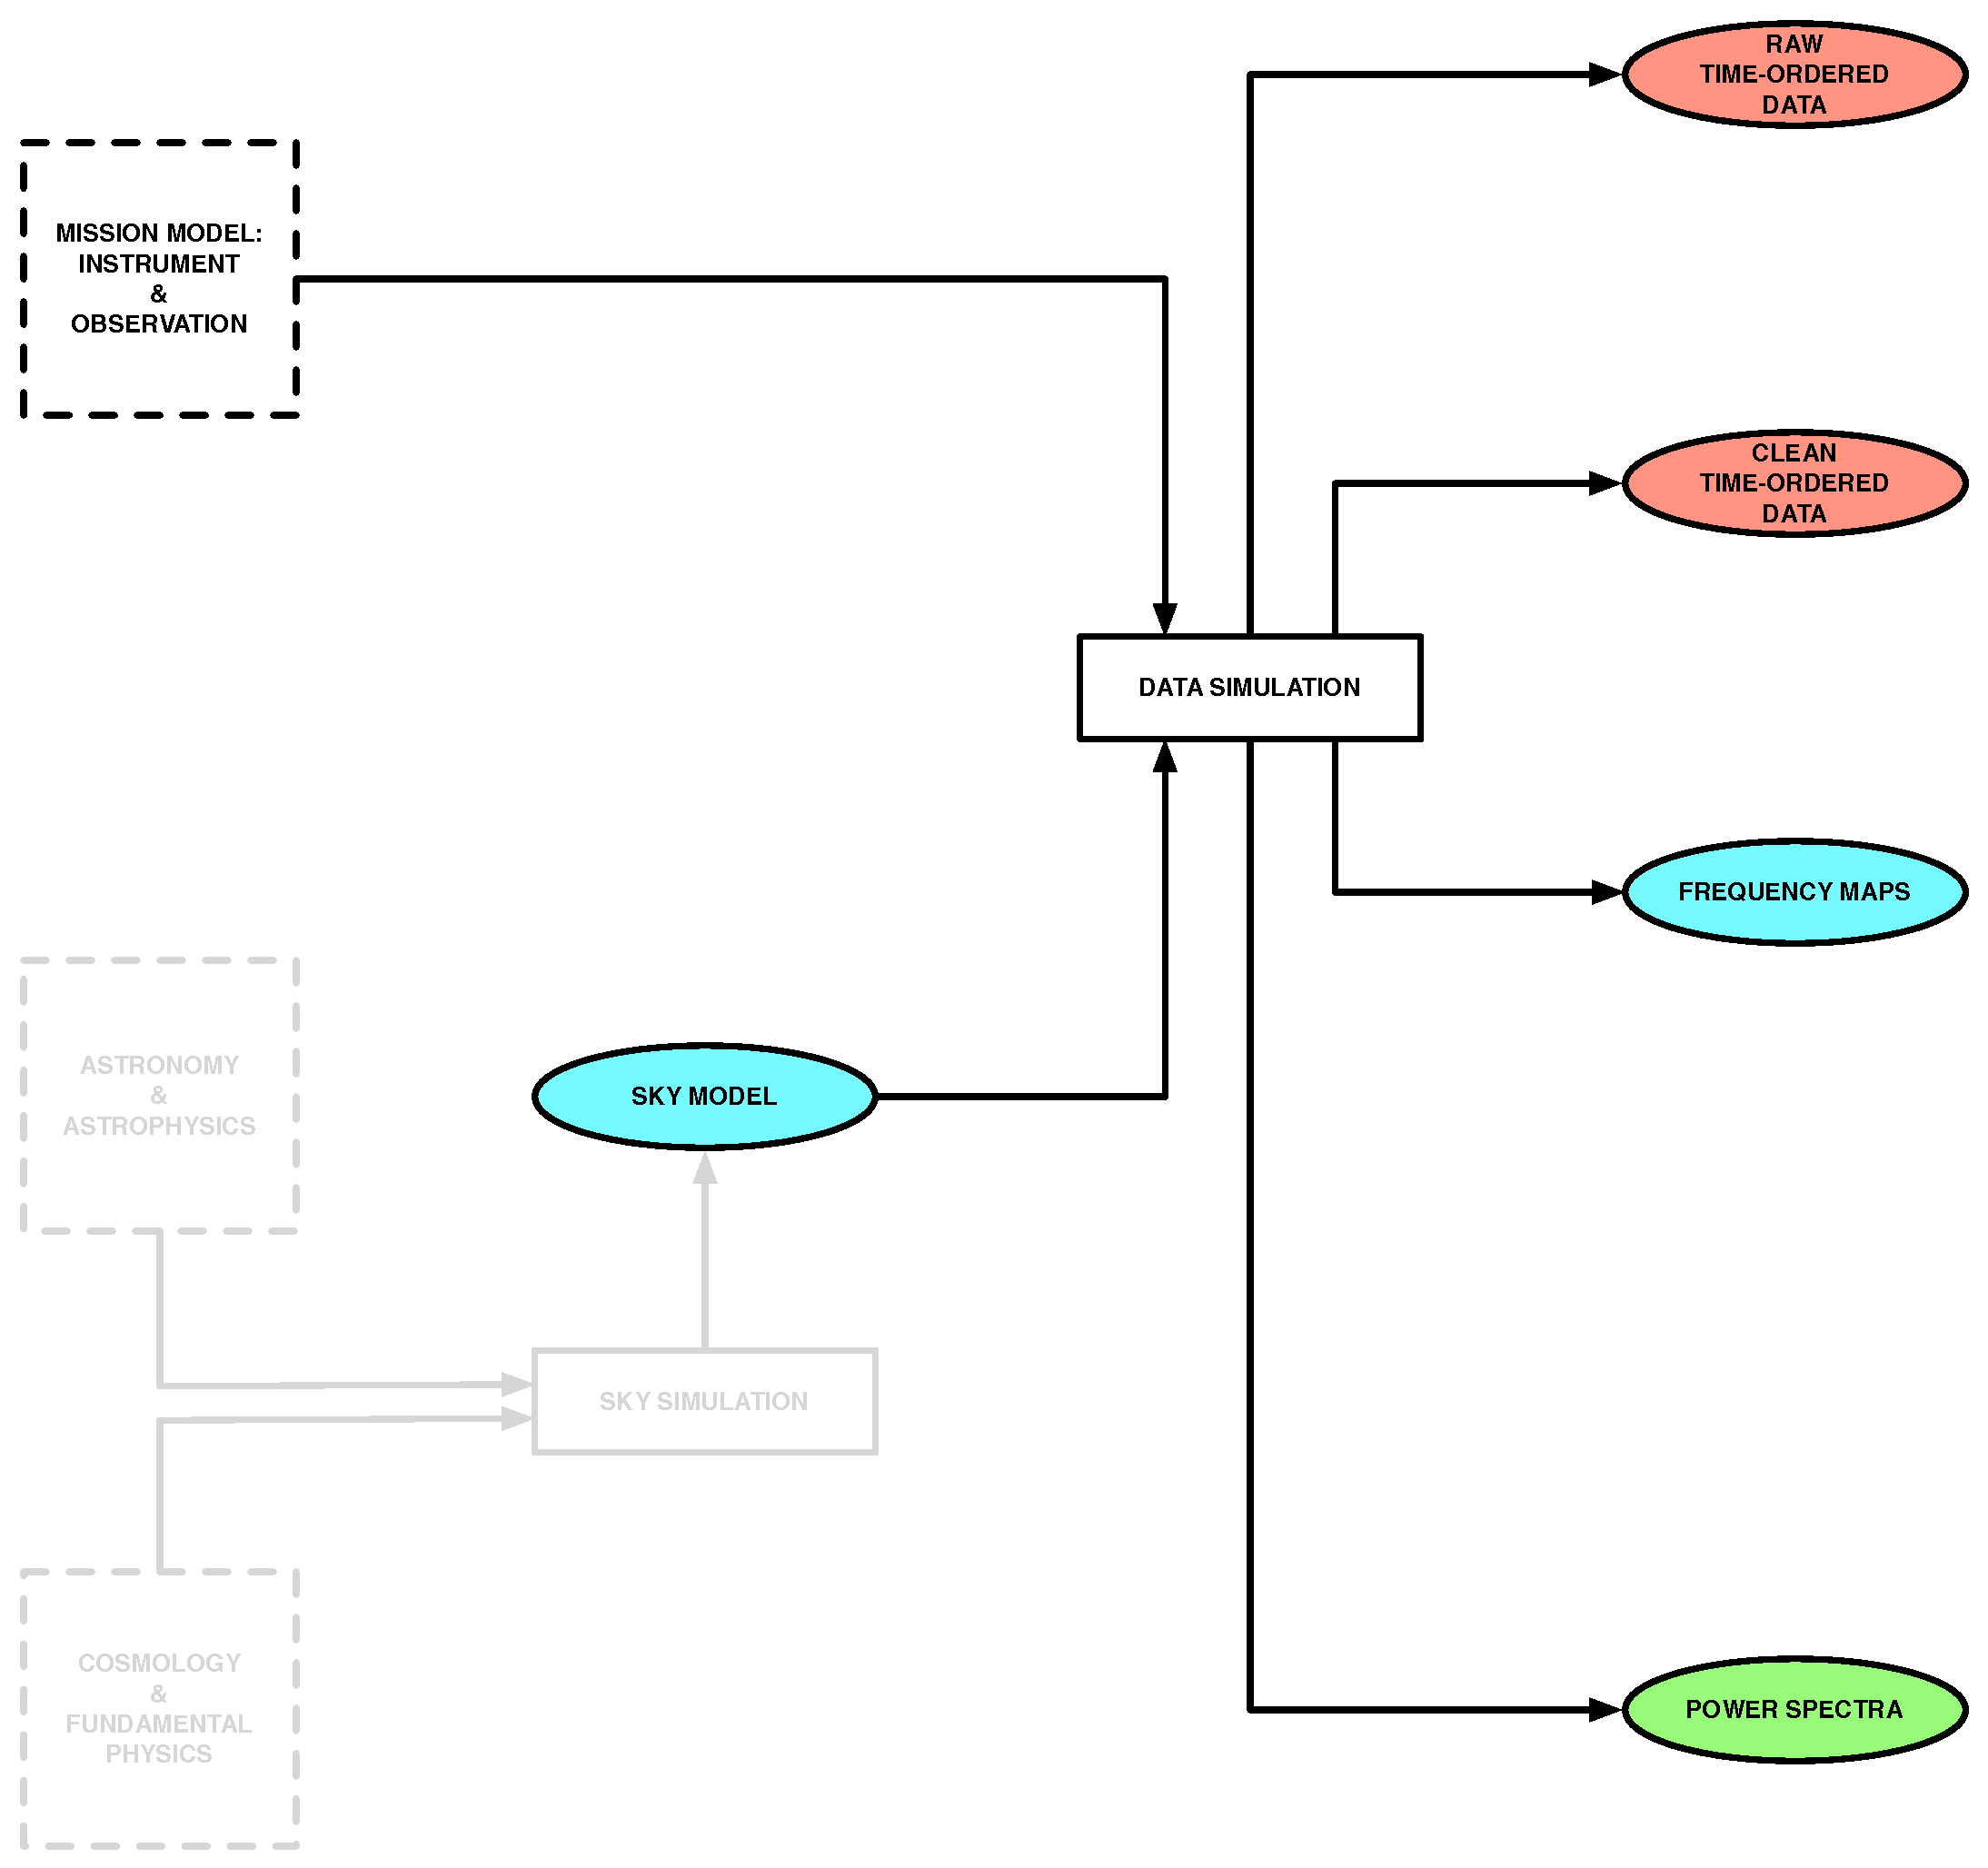
\includegraphics[width=1\textwidth]{Analysis/ds}
\caption{The data simulation subset of the CMB simulation pipeline}
\label{fig_ds}
\end{figure}

At the most detailed level, the observation model includes the telescope pointing (typically sampled more sparsely that the detectors), and its environment (comprising the atmosphere and surroundings for a ground-based telescope). Correspondingly, the instrument model includes each detector's polarized $4 \pi$-beam and bandpass (defining the optical power incident on the detector for a given pointing), and a model of its electronics and readout (defining the recorded output data resulting from that optical power).

\subsection{Time Domain}

TOD simulations are necesserily the most expensive to perform, but provide the most precise representation of the mission data. In particular they enable the injection of systematic effects into the data both to assess strategies for their removal and quantify and residuals.

For a given detector, we first reconstruct the detector pointing (including any polarization modulation) from the overall telescope pointing model. We then generate the astrophysical sky signal for each pointing by convolving the sky model map with the beam and bandpass. The astrophysical sky signal is added to additional simulated signals from stray light, atmospheric signal fluctuations, and ground pickup, and the total signal is propagated through a simple simulation of the optics to include the polarization angle rotations and optical efficiencies of the optical stages. This results in a simulated  time ordered data set of the total millimeter-wave power incident on the detector.

For a clean TOD simulation this is sufficient; however for a raw TOD we now need to apply a physical model of the detector system and associated readout to convert the optical power into detector output. The details of the physical model depend on the detector technology, but as an example we consider a transition-edge superconducting (TES) bolometer read out with a multiplexed SQUID amplifier. The simulation would then need to model the flow of heat in the TES absorber and the flow of current and magnetic flux through the SQUID readout. Variations in ambient magnetic field could also be added at this stage. Such a simulation would also need to incorporate detector-detector correlations induced by crosstalk or thermal fluctuations.  Additional filters applied by the readout electronics would also be included, including digitization with an analog to digital converter. For MKID or coherent receivers, the physical model would be different in detail, but would include a similarly detailed model.

%% Map/spectral domain text lifted from forecasting section?

\subsection{Map Domain}

Effective beam convolution (map domain via time domain pointing)


\subsection{Spectral Domain}

%\bibliography{cmbs4}

%%
%% Populate the .bib file with entries from SPIRES Bibtex (preferred)
%% or ADS Bibtex (if no SPIRES entry).
%%  SPIRES will also supply the CITATION line information; please include it.
%%


